\chapter{State of the Art}

The State-of-the-Art consists in exposing the highest level of development regarding the topics related to this bachelor thesis. This section helps having a common ground between the reader and the writer as to what the key concepts are, as lot of the design decisions are based on these concepts.

The section \ref{chapter2_operating_system} in dedicated to introducing the concepts of operating systems and its relevant features.

In the section \ref{chapter2_armv6}, we introduce the basics of the ARMv6, that is, its architecture, registers, CPU modes, etc.

The section \ref{chapter2_serial_communications} presents serial communications and a protocol over this method: The UART.

The last section, \ref{chapter2_raspberry_pi} is aimed to present what is relevant to know regarding the Raspberry Pi from a development perspective.

\section{Operating System}\label{chapter2_operating_system}

OS are designed to handle real-time application to process data as it comes in. The RTOS group of OS includes real-time processing time and response time requirements.
The main characteristics of the RTOS are the following:
\begin{itemize}
\item\textbf{Jitter:} The jitter is the deviation from true periodicity of a presumed periodic signal. In the context of RTOS, the jitter is the deviation of the deadline of the system in respect to the deadline expected\cite{chibios_jitter}.
\item\textbf{Scheduling algorithm:} This is how the system will determine the next process to be executed and how it will execute. The more famous algorithm are the pre-emptive algorithms, the more famous being \textit{Round Robin (RR)}, \textit{Fixed priority pre-emptive scheduler}. Other non-pre-emptive algorithms can be \textit{Earliest Deadline First} and \textit{FIFO}.
\item\textbf{Interrupt latency} The interrupt latency is defined as: "the time that elapses from when an interrupt is generated to when the source of the interrupt is serviced". This depends on a lot of criteria such as the time of interruption (synchronous or asynchronous), the processor architecture as well as the interrupt masking (interrupt enabled or disabled) and the interrupt handler (depends on the OS).
\item\textbf{Context and thread switch latency:} Thread switching is the process of storing and restoring the state of a thread and saving restoring another one. This creates the illusion of simultaneous threads executing at the same time while in fact, all the threads are executing sequentially but a context switch is done many times a second. The time needed to store the state of a thread and restore another thread is the thread switch latency. This depends on many things such as the Task scheduler (including how fast the scheduling algorithm is), whether threads are part of same process (if not, CPU cache overhead are to be expected), the architecture of the CPU as well as the data structure used for the context switching itself.
\end{itemize}


What enters in consideration while using an OS is the different inter-task communication that it offers. Intertask Communication is a possibility to share resources amongst different tasks (thread or process). The more popular method are:
\begin{itemize}
\item\textbf{Disabling interrupts:} This is the most basic resource sharing method. When a critical resource is used and cannot be accessed at the same time, interrupts are disabled in order to avoid any interruptions of the execution flow until the sections related to the resource is over. This is the simplest way to avoid having two processes from accessing a critical section at the same time.
\item\textbf{Mutexes:} This method is a lot more costly CPU-cycle wise than simply disabling interrupts. It uses the analogy of a traffic light: When a developer knows that a thread reaches a critical section, the thread is to poll the mutex so as to check for resource availability. If the mutex is disabled, the resource is being accessed by another thread. When the mutex is available, the thread disable the mutex, accesses the resource, and when it goes out of the resource re-enables the mutex.
\item\textbf{Semaphore:} This is the generalisation of the mutex: The difference with the mutex is that a semaphore can allow several threads to access the critical sections and get disabled once the maximum number of thread accessing the critical section at the same time has been reached.
\item\textbf{Message passing:} In this paradigm, there's only one owner of a resource, when other threads want to access or get information regarding this resource, it ask first to the owner the right to do so, then the owner can grant, delay or deny the access of the resource.
\item\textbf{Synchronous message passing:} The sender thread sends a message to the receiver thread, the sender needs to wait the sender to receive such message, which can result in a very inefficient method.
\item\textbf{Queues:} This is the asynchronous flavour of the previous bullet point: A message is sent by a sender but it doesn't wait for the receiver to receive the message, instead, the execution flow of the sender continues. However, a problem can arise when a sender continues the execution flow without the receive completely received the message. This is why queue are used as a message passing buffer that can be accessed asynchronously.
\end{itemize}


OS are expected to handle the starting and finishing of a program, that is, the OS doesn't know beforehand its execution what the program that it will have to handle will be.
OS have emerged as an important discipline in Computer Science due to the increasing in computational power, An OS proposes flexibility for the software by providing tools to the developer. POSIX has a categories for the special case of OS, RTOS, named POSIX.1b, witnessing the importance in the industry of such class of OS. Dennis M. Ritchie made a very interesting paper\cite{ritchie_UNIX} in 1974 where he present the UNIX operating system as well as several key components such as: a hierarchical file system, inter-processes or even an asynchronous process initialization. UNIX has played a key role in the development of modern operating systems.


\section{ARMv6} \label{chapter2_armv6}
As explained before, ARM is especially suited for embedded systems and systems that are required to be power efficient. The ARMv6, is the architecture the one that we are interested in as the CPU used in the Raspberry Pi B+ is a 32-bits ARM1176JZF-S. A description of the the different properties of this architecture is described below.

\subsection{CPU modes}
The ARMv6 architecture presents different CPU modes, that is, modes with different privileges and dedicated registers. When the devices starts, the device is set into privileged mode, that means that it can write in almost all the registers and change execution mode. At any given time, the processor can only execute in one given mode, however, externals events (exceptions or instructions) can trigger an execution mode change. There's basically one CPU mode per type of exception:

\begin{itemize}
\item\textbf{User mode:} This is the mode with the least privilege, this is the mode the CPU should be in when executing user programs.
\item\textbf{Interrupt Request (IRQ)}
\item\textbf{Fast Interrupt Request (FIQ)}
\item\textbf{Supervisor (SVC)} Privilege mode when CPU is reset or when switching using the dedicated instruction
\item\textbf{Abort mode} Privilege mode when a prefetch abort exception or data abort exception has been thrown.
\item\textbf{Undefined mode} Privilege mode when an undefined instruction exception has been thrown.
\item\textbf{System mode} Privilege mode only accessible from the dedicated instruction by modifying the CPSR
\end{itemize}


\subsection{Interrupt vector table}
The interrupt vector table (and therefore the interrupt vectors) are very important part of the interruption process. While receiving an interruption, the processor save the current program pointer and stack pointer, switches to the adequate CPU mode and branches to the appropriate interrupt vector. The vector table associates the interrupt handler with the interrupt request so that the processor knows what part of the code to execute to handle a particular interrupt.

As a result, it is required to define an interrupt handler for each of the possible interruption. Below is a table displaying the list of interrupt that may arise during code execution along with their CPU mode:

\begin{table}[H]
    \centering
    \begin{tabular}{| p{3cm} | p{7cm} |}
    \hline
    \textbf{CPU Mode}	&  \textbf{Interruption} \\ \hline
    Abort              &  \textbf{Reset}: Reset triggered by the watchdog. Also, first interruption triggered while booting the kernel. \\ \hline
    Abort              &  \textbf{Prefetch Abort}: Instruction couldn't be prefetched correctly \\ \hline
    Abort              &  \textbf{Data Abort}: Data abort interrupt can be caused by many reasons such as alignment faults, translation faults or access bit faults. \\ \hline
    Undefined          &  \textbf{Undefined Instruction}: Undefined instruction found during the execution. This can be used to extend the ARM instruction set by creating new instruction handled by this interruption handler. \\ \hline
    IRQ 				&  \textbf{Software Interrupt}: Synchronous interruption handler generated by the code, for instance, when using a system call. \\ \hline
    IRQ                &  \textbf{Hardware Interrupt}: Asychronous interruption handler generated by the hardwhare, for instance, via I/O or timer interruption. \\ \hline
    FIQ                &  \textbf{Fast Interrupt}: Higher priority interruption than software interrupt.\\ \hline
    \end{tabular}
    \caption{Message structure to obtain a frame-buffer from the VideoCore}
\end{table}


\subsection{Registers}
The ARM architecture specifications specifies \textit{37 registers}:
\begin{itemize}
\item Thirteen general-purpose registers namely R0-R12
\item One Stack Pointer (SP) per mode. This register can also be named R13.
\item One Link Pointer (LR) per mode. This register can also be named R14.
\item One Program Counter (PC)
\item One Current Program Status Register (CSPR).
\end{itemize}

A register is qualified as \textit{banked} when the mode can use these registers without needing to restore their initial value. As there are one SP and LR registers for each mode, SP and LR are therefore banked registers in every mode. R0 to R12 are never banked registers on the exception to the FIQ mode where R8 to R12 are banked.
The figure~\ref{fig:chapter2_registers_vs_modes} borrowed from the the ARM documentation summarizes the registers versus modes relation.

\begin{figure}[H]
\begin{center}
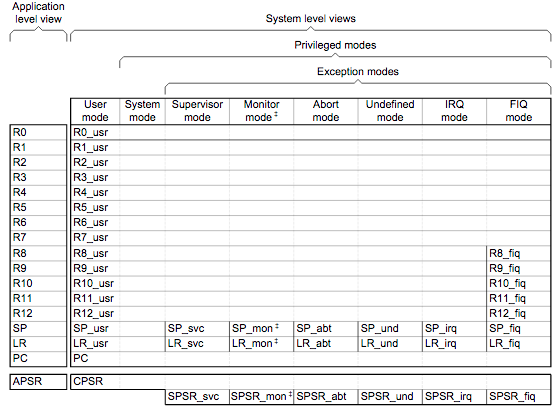
\includegraphics[width=1\textwidth]{includes/figures/chapter2_registers_vs_modes.png}  \\[0.5 cm]
\end{center}
\caption{Registers and Modes summary}
\label{fig:chapter2_registers_vs_modes}
\end{figure}


As explained before, the CPSR is the main register to use for switching state. But in fact, the CPSR is used for a lot more than just mode switching, it has (amongst other) these uses: 

\begin{itemize}
\item Processor mode
\item Thumb enabled/disabled bit
\item FIQ enabled/disabled bit
\item IRQ enabled/disabled bit
\item Data endianness bit
\item Branch state bit (namely IT)
\item Greater-than-or-equal-to bit (namely GE)
\item Do-not-monidify bits (DNM)
\item Carry/borrow/extend bit
\item Zero bit
\item Negative/less than bit
\end{itemize}

This is why it is extremely important to be careful when modifying the CPSR, this is why the ARM is also provided with a SPSR. Also, it is prime importance to save such register when performing context switching. Finally, the CPSR contains reserved bit, as explained in the ARM documentation these registers are currently unused but present for future features. The figure~\ref{fig:chapter2_cpsr} pictures a summary of the bits present in the CPSR in a graphical manner.

\begin{figure}[H]
\begin{center}
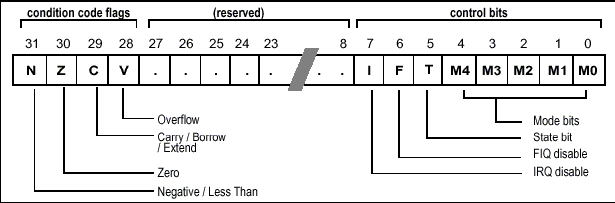
\includegraphics[width=1\textwidth]{includes/figures/chapter2_cpsr.png}  \\[0.5 cm]
\end{center}
\caption{CPSR bits}
\label{fig:chapter2_cpsr}
\end{figure}


\section{Serial Communications}\label{chapter2_serial_communications}
\subsection{Introduction}
The serial communication (as opposed to parallel communication) is the process of sending data one bit a time over a communication channel. This is one of the simplest mean of communication and one of the more used in mainstream computing as for instance USB, SATA and PCIe are all using serial communication within their protocol. The serial communication uses a series of mechanisms that provide error-free transfers across the devices such as synchronization bits (to avoid data loss) and parity bits (for error checking).

Serial communications are all based on a internal clock that has to be known before starting the communication that is called the \emph{baud rate}. The baud (in bits per seconds) specifies how fast data is sent over the serial communication. It is important to know beforehand the baud rate of the communication otherwise it is impossible for the two devices to synchronize and exchange data without errors.

The serial communication being just a concept, the specifics of the protocol such as data framing, synchronization, error checking, etc. are specified by the standard used. The one used in this project is specified in the next section.


\subsection{UART}
UART stands for \textit{Universal Asynchronous Receiver/Transmitter}\cite{uart} and is a computer devices that is used to translate data sent from a parallel way into byte and vice versa. It is therefore required that both ends of the link have a UART devices in order to be able to communicate.

As for many other protocols, UART uses frames to transmit its data, that is, the data that is to be transferred is cut into little chunk which are framed (i.e. placed into sequence of a bit data allows the receiver to know where the boundaries of the data are).
The frame contains:
\begin{itemize}
\item A start bit
\item The data
\item Parity bit (optional)
\item Two stop bits
\end{itemize}

When the communication is idle, all the bits are set HIGH, it therefore comes that the start bit is set to LOW. The parity bit is optional but provide an additional layer of error checking. Finally, the two stop bits are always set to HIGH.


\begin{figure}[H]
\begin{center}
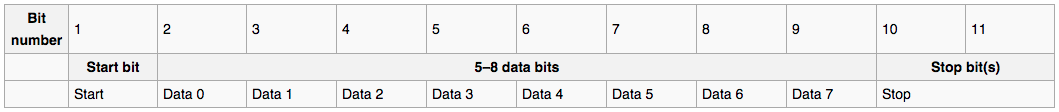
\includegraphics[width=1\textwidth]{includes/figures/chapter2_uart_framing.png}  \\[0.5 cm]
\caption{Schema of a frame in a UART transmission}
\end{center}
\label{fig:chapter2_uart_framing}
\end{figure}

 



\section{Raspberry Pi B+}\label{chapter2_raspberry_pi}
On top of the ARM resides the Raspberry Pi with its set of rules and hardware. For this section, we will focus on the model that is relevant for this project, that is, the Raspberry Pi model B+.

\subsection{Hardware}
The hardware has to be handled by the kernel up to a certain extends. Depending on the hardware, different parameters parameters and protocols are to be employed. This section is a summary of the relevant part of how to use them and how it has been design in the kernel.

In order to gather the information related to a given hardware, the official Broadcom BCM2835 ARM Peripherals manual\cite{arm_peripherals_manual} has be used. It states on page 6:

\begin{displayquote}
Physical addresses range from 0x20000000 to 0x20FFFFFF for peripherals. The bus addresses for peripherals are set up to map onto the peripheral bus address range starting at 0x7E000000. Thus a peripheral advertised here at bus address 0x7Ennnnnn is available at physical address 0x20nnnnnn.
\end{displayquote}

We are going to use the physical address (i.e. from 0x20000000 to 0x20FFFFFF). The peripheral address of the Raspbery Pi can be found with an offset from the base value. For instance, the GPIO address can be found with an offset of 0x200000, the UART with an offset of 0x201000, etc).

The hardware in the scope of this bachelor thesis are the GPIO, the UART and the GPU. We will therefore introduce these components below.

\subsubsection{GPIO}
The GPIO is the easiest way to handles I/O with an external devices, as its name implies. The Raspberry Pi uses a J8 header, that is, a 26-usable-pins GPIO, the other being for the ground or power supply. Finally, there are some GPIO numbers that don't have any physical pins but have influence on the board. For instance, GPIO 47 refers to the ACT LED. The figure~\ref{fig:chapter2_GPIO_pins} is a table presenting the GPIO pins\cite{pi4j}.

\begin{figure}[H]
\begin{center}
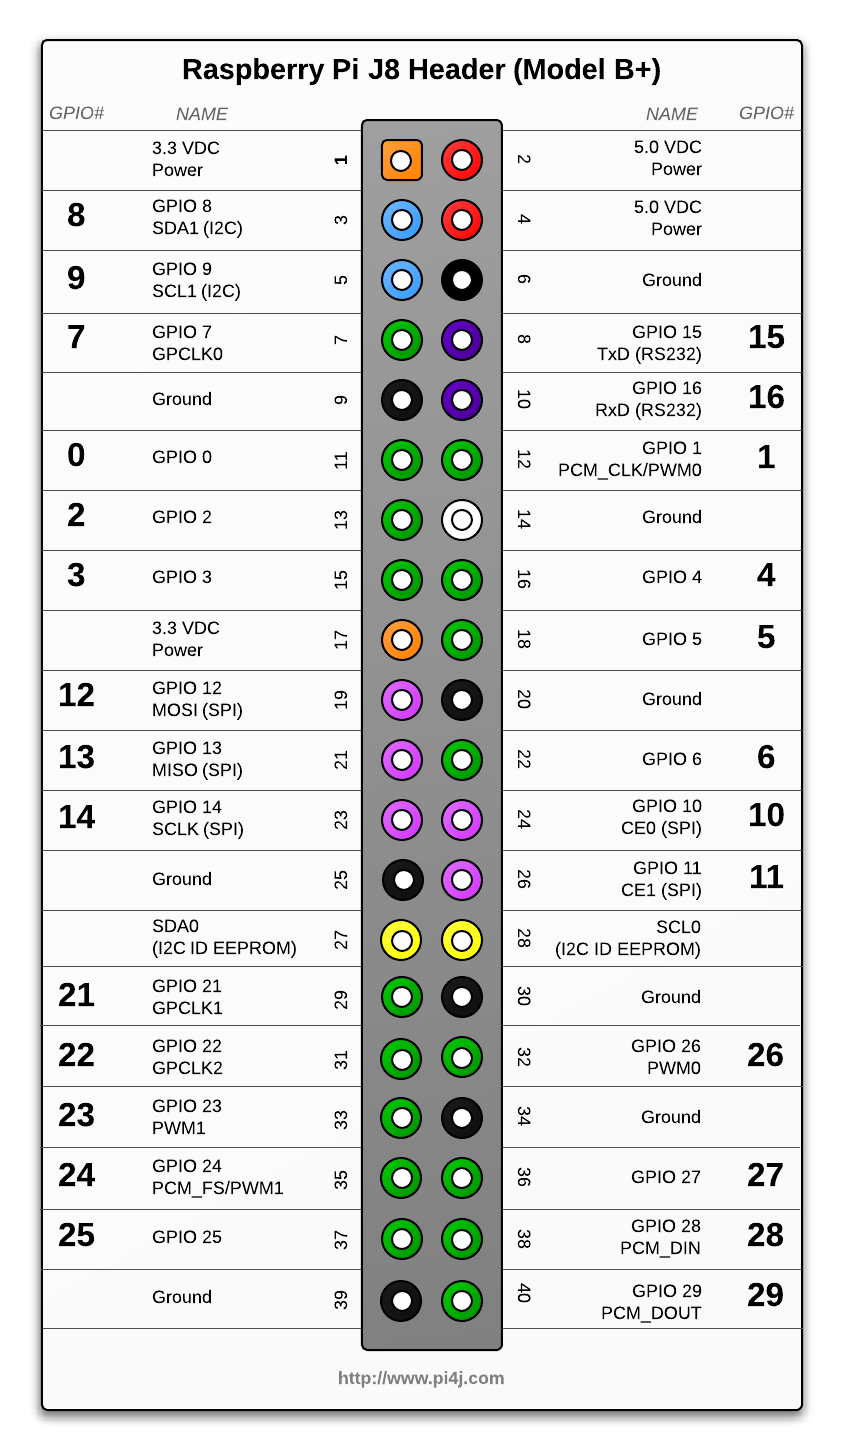
\includegraphics[width=0.4\textwidth]{includes/figures/chapter2_GPIO_pins.png}  \\[0.5 cm]
\end{center}
\caption{GPIO pins of the Raspbery Pi B+}
\label{fig:chapter2_GPIO_pins}
\end{figure}

Only five pins are actually used for the project:
\begin{itemize}
\item\textbf{Pin 2 - 5.0V DC} - This will be the Pin used for providing power to the board.
\item\textbf{Pin 6 - GROUND}
\item\textbf{Pin 8 - TxD} - Transmit data. This is the pin used to output data serially to the computer.
\item\textbf{Pin 10 - RxD} - Receive data. This is the pin used to receive data serially from the computer.
\item\textbf{Pin 47 - ACT LED} - It is possible to turn it on and off, this led is specially useful before having implemented the serial output drivers.
\end{itemize}


The pins 8 and 10 are used for the UART serial communication between the computer and the Raspberry Pi.

\subsubsection{The Message-Handling Unit: The Mailbox}

The mailboxes\cite{mailbox} are a hardware tool that ease the communication between the the ARM processor and the VideoCore. It allows the communication of these two components using asynchronous messages, hence the name 'Mailbox'. It contains seven channels that are each for a different purpose/task:
\begin{itemize}
	\item\textbf{Channel 0}: Power management interface channel
	\item\textbf{Channel 1}: Frame-buffer channel
	\item\textbf{Channel 2}: Virtual UART channel
	\item\textbf{Channel 3}: VCHIQ interface
	\item\textbf{Channel 4}: LEDs interface channel
	\item\textbf{Channel 5}: Buttons interface channel
	\item\textbf{Channel 6}: Touch-screen interface channel
\end{itemize}

All of these mailbox can contain up to \textit{height} messages of 32-bits which can be allocated using a FIFO policy.

The only channel that we will be using for this work is the channel 1, related to the frame-buffer as it will help us to ask for the VideoCore a address where the data related to the screen can be written. Please find the status of the organization of the message hereunder:

\begin{table}[H]
    \centering
    \begin{tabular}{| p{3cm} | p{7cm} |}
    \hline
    \textbf{Byte}	&  \textbf{Meaning} \\ \hline
        0                   &  \textbf{Physical Width}: Width to upscale the virtual width to. \\ \hline
    4                   &  \textbf{Physical Height}: Height to upscale the virtual height to. \\ \hline
    8                   &  \textbf{Virtual Width}: Width of the native frame-buffer \\ \hline
    12                  &  \textbf{Virtual Height}: Height of the native frame-buffer \\ \hline
    16                  &  \textbf{GPU - Pitch} \\ \hline
    20                  &  \textbf{Bit Depth}: How many byte to allocate for each pixel, related to colour depth \\ \hline
    24                  &  \textbf{X}: Number of bits to skip in the top left side on the horizontal axis \\ \hline
    28                  &  \textbf{Y}: Number of bits to skip in the top left side on the vertical axis \\ \hline
    32                  &  \textbf{GPU - Pointer}: Pointer where the frame-buffer is located\\ \hline
    36                  &  \textbf{GPU - Size}: Size of the the frame-buffer in byte\\ \hline
    \end{tabular}
    \caption{Message structure to obtain a frame-buffer from the VideoCore}
\end{table}



\subsection{Booting Process}\label{chapter2_booting_process}
The board is devoid of power button, instead, the Raspberry Pi boots automatically when power is applied to the board. The booting process is a bit atypical as the device that is first powered and that initializes the booting sequence is the VideoCore processor, which start the stage 1 bootstrap from the ROM in the SoC. The stage 1 bootstrap gives the instruction to initialize the SD Card, mount it and start the file bootcode.bin. 
Below is the list of the boot stages:
\begin{enumerate}
  \item\textbf{hardcoded firmware} - This code starts on the GPU, mounts and executes stage 2.
  \item\textbf{bootcode.bin} - Still running on the GPU, it enables the RAM and starts stage 3.
  \item\textbf{start.elf} - This is the firmware of the GPU. It reads the file \textit{config.txt} if any, and starts setting up the GPU. This stage is also in charge of partitioning the RAM into two regions: GPU RAM and CPU RAM, this is set so that the ARM processor will take the leftover RAM. It finally reads another configuration file: \textit{cmdline.txt}, it contains the attributes to be passed to the kernel before starting. Finally, it loads and execute the kernel.img file and start the CPU.
  \item\textbf{kernel.img} - This is the user code, that is, the file that this thesis aims to produce.
\end{enumerate}


Both \textit{bootcode.bin} and \textit{start.elf} can be found on the official repository of the Raspberry Pi\cite{firmware_boot} but they belong to BroadCom that hasn't released the source for those two files and have various feature that are undocumented, which makes custom boot-loaders extremely tedious to produce.

This is the latter that we will implement. It is to be compiled with the arm cross compiler\cite{osdev_raspberry_pi}.

\begin{figure}[H]
\begin{center}
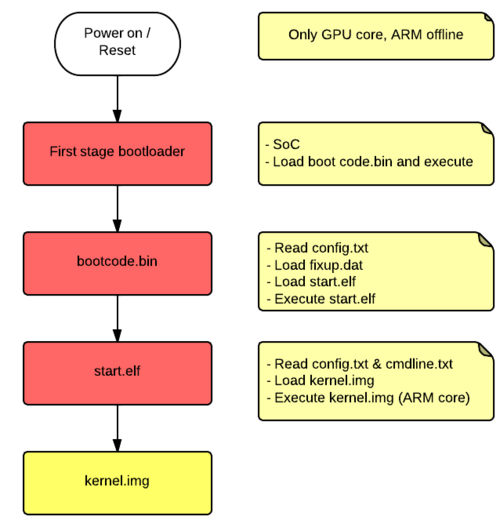
\includegraphics[width=0.5\textwidth]{includes/figures/chapter1_booting_process.png}  \\[0.5 cm]
\caption{Schema representing the boot process}
\end{center}
\end{figure}

\subsubsection{config.txt}
As aforementioned, this file contains parameters that are used to set up the CPU and GPU. A broad range of parameters can be set\cite{config_txt}: from the memory that the GPU will use, disable or enabling the L2 cache, setting up the audio and PWM, setting up the HDMI video mode (video, audio, frequency, resolution, pixel encoding, etc.).

\subsubsection{kernel.img}
This is the user code. The bootloader stage 3 will load that file and by default expect the first instruction to be stored at the address \textit{0x8000}, this is to be taken into account when compiling our kernel.

\subsection{Famous Operating Systems}
Not surprisingly, the most popular OS' on the Raspberry are Linux-based. Here is a non-exhaustive list of the most notable operating system that can be run by the Raspberry Pi:
\begin{itemize}
\item\textbf{Raspbian\cite{raspbian}:} OS based on the highly popular Debian distribution optimized for the Raspberry-Pi. Raspbian is bundled with more than 35000 packages, which allow a very broad set of possibilities (from Desktop use to more specific use for developers. This is the go-to OS for a general purpose Raspberry Pi.

\item\textbf{ArchLinux\cite{archlinux_arm}:} Port of the ArchLinux distribution to ARM processors. It is suited for more specific use as the user can and has to install specific packages that is suited for its use as the basic installation only comes with the Linux kernel, a shell and a package manager.

\item\textbf{OpenELEC\cite{openelec}:} OpenELEC stands for \textit{Open Embedded Linux Entertainment Center}, this is the go-to distribution for using the Raspberry Pi as a media center.

\item\textbf{Kali Linux\cite{kali}:} As for ArchLinux, this is a port of the popular Kali Linux to the ARM processors. This is the distribution of choice for forensics analysis and penetration testing.

\item\textbf{RetroPie\cite{retropie}:}  This distribution is for entertainment purposes as it proposes a wide set of emulator for old consoles proposing a retro gaming experience. The distribution supports game pads for various consoles as long as an adapter is purchased.

\item\textbf{FreeRTOS\cite{freertos}:} Whereas the previous OS are all based on the Linux Kernel, FreeRTOS has its standalone kernel and Operating System specially tailored for real-time purposed for embedded systems
\end{itemize}


\subsection{Raspberry Pi in the Scientific Literature}

Mr \textit{Eric Biggers} wrote a paper regarding the port of Xinu\cite{xinu_biggers}, an Operating System totally independent on UNIX as it has been made without any goal of compatibility and without the knowledge of the source code of UNIX. The paper shows different challenges and solutions brought by Mr. Biggers in order to port it to the Raspberry Pi. Other papers have been publish but are more related to the IoT\footnote{Internet of Things}, it is therefore out of the scope of this document.
